%% Beispiel-Präsentation mit LaTeX Beamer im KIT-Design
%% entsprechend den Gestaltungsrichtlinien vom Februar 2025
%%
%% Siehe https://sdq.kastel.kit.edu/wiki/Dokumentvorlagen

%% Beispiel-Präsentation
\documentclass{sdqbeamer}[en]
 
%% Gruppenlogo, muss im Verzeichnis logos/ liegen
%% falls kein Gruppenlogo gewünscht, bitte \grouplogo{} aufrufen
\grouplogo{codex_logo} 

%% Gruppenname und Breite (Standard: 89 mm)
\groupname{ITEC - Institute of Computer Engineering}
%\groupnamewidth{89mm}

% Beginn der Präsentation

\title[Requirements Analysis]{CodeX: Natural Language to Structured Code Generation}
\subtitle{Requirements Analysis} 
\author[Dayana Karadzhova]{Oleksandr Brittner, Simon Bumiller, Simon Gaber, \textbf{Dayana Karadzhova}, Kyrylo Pavlov \newline}

\date[5.\,12.\,2025]{December 5, 2025}

% Literatur 
 
%\usepackage[citestyle=authoryear,bibstyle=numeric,hyperref,backend=biber]{biblatex}
%\addbibresource{presentation.bib}
%\bibhang1em

\usepackage{lipsum}

\usepackage{pdfpages}

% Config for listings
\usepackage{listings}
\lstdefinelanguage{Chef}{
  sensitive=true,
  morekeywords={Ingredients,Method,Put,Take,Fold,Add,Subtract,Serve,Label,If,goto},
}
\lstset{
  basicstyle=\ttfamily\small,
  keywordstyle=\bfseries,
  columns=fullflexible,
  breaklines=true
}

% Custom commands for requirements
\newcommand<>{\must}[2]{%
  \uncover#3{{$\langle RM#1\rangle$} #2\\}%
}
\newcommand<>{\should}[2]{%
  \uncover#3{{$\langle RS#1\rangle$} #2\\}%
}
\newcommand<>{\could}[2]{%
  \uncover#3{{$\langle RC#1\rangle$} #2\\}%
}
\newcommand<>{\qualityReq}[2]{%
  \uncover#3{{$\langle Q#1\rangle$} #2\\}%
}


\begin{document}

%Titelseite
%\begin{frame}[title white vertical, picture=images/palladio_bauplan]
%	\titlepage
%\end{frame}

%\begin{frame}[title blue vertical, picture=images/palladio_bauplan]
%	\titlepage
%\end{frame}

\begin{frame}[title green horizontal, picture=images/circuit, kitlogo=white]
\titlepage
\end{frame}

%\begin{frame}[title white horizontal, picture=images/palladio_bauplan, kitlogo=white]
%\titlepage
%\end{frame}

%Inhaltsverzeichnis
\begin{frame}[tableofcontents=green]{Content}
	\tableofcontents
\end{frame}

%\begin{frame}[tableofcontents=blue]{Inhaltsverzeichnis}
%	\tableofcontents
%\end{frame}

\section{Motivation}

\begin{frame}[t]{Motivation}{Example: Chef Programming Language}
\begin{itemize}
    \item Created 2002 as an esoteric and stack-based programming language
    \item Similarities to \textit{Shakespeare} or \textit{BASIC}
    \item<2-> Not used in actual projects
    \item<2-> Therefore, code-examples are missing in training data of \textit{LLM}s
\end{itemize}
\end{frame}

\begin{frame}[fragile]{Motivation}{Example: Chef Programming Language}


\begin{columns}
\begin{column}{0.5\textwidth}
Response from \textit{ChatGPT} for the prompt \textit{"Create a program in the chef programming language for computing fibonacci numbers without comments."}:
\vspace{1.0em}
\begin{lstlisting}[basicstyle=\ttfamily\scriptsize,language=Chef]
Fibonacci Calculator

Ingredients.
10 g n
0 g a
1 g b
0 g temp

Method.
Put n into mixing bowl.
Fold a into mixing bowl.
Fold b into mixing bowl.
Label start.
Take a from mixing bowl.
Take b from mixing bowl.
Add a to b.
Put b into temp.
Put b into a.
Put temp into b.
Take n from mixing bowl.
Subtract 1 from n.
Put n into mixing bowl.
If n > 0, goto start.

Serve with a.
\end{lstlisting}
\end{column}
\begin{column}{0.5\textwidth}
    \begin{center}
        \begin{itemize}
            \item<2-> Basic code structure is correct: \textbf{Ingredients}, \textbf{Method.} and \textbf{Serve} directives.
            \item<3-> However: \textbf{Label} and \textbf{goto} do not exist.
            \item<4-> Due to low prevalence in training data, \textit{ChatGPT} can't create correct code samples for niche languages $\rightarrow$ RAG helps us solve this problem.
        \end{itemize}
    \end{center}
\end{column}
\end{columns}

\end{frame}

\section{Requirements}

\begin{frame}[t]{Minimum requirements}
    \must{1}{The system must provide a web interface that allows to convert natural language into a snipped of code. The target \textit{\hyperref[abr:DSL]{DSL}} can be selected out of options, and the generated code can be exported as a file.}
    \vspace{0.5em}
    \must{2}<2->{The system must provide \textit{\hyperref[abr:SPICE]{SPICE}} as one option of it's selectable \textit{\hyperref[abr:DSL]{DSL}s}.}
    \vspace{0.5em}
    \must{3}<3->{\textit{\hyperref[abr:SPICE]{SPICE}} conversations must have a visualization of the respective circuit.}
    \vspace{0.5em}
    \must{4}<4->{Every conversation must have a name.}
    \vspace{0.5em}
    \must{5}<5->{The system must support the requests to the \textit{\hyperref[abr:LLM]{LLM}} using a \textbf{\hyperref[abr:RAG]{RAG}} approach. The data that is retrieved must be stored on a secure database that respects \textbf{\hyperref[abr:IP]{IP} property}.}
    \vspace{0.5em}
    \must{6}<6->{The system must integrate a validation backend to validate the generated circuit for \textit{\hyperref[abr:SPICE]{SPICE}} conversations.}
    \vspace{0.5em}
    \must{7}<7->{The system must allow adding/removing seperate \textit{\hyperref[abr:LLM]{LLM}} models together with their \textit{OpenAI API} URL. When a request is made, the user should be able to select the model with which the request will be performed.}
\end{frame}

\begin{frame}[t]{Optional Requirements}{User accounts}
    \should{3}{Users can sign up, login and logout of accounts using a username (or email) and password.}
    \vspace{0.5em}
    \should<2->{5}{The system should allow users to securely update their email, username and profile picture.}
    \vspace{0.5em}
    \could<3->{9}{During registration, the user's email could be confirmed by sending a verification link or code. Registration would not be completed until the email is confirmed. When the user would change their email, a new email confirmation would automatically be issued.}
    \vspace{0.5em}
    \could<4->{17}{Users could upload and display a profile picture associated with their account.}
\end{frame}

\begin{frame}[t]{Optional Requirements}{Admin role}
    \could{4}{Every account could be associated to one of the roles \textbf{\hyperref[def:admin]{Admin}}, \textbf{\hyperref[def:user]{User}} or \textbf{\hyperref[def:guest]{Guest}}. Every role could have a specified upper bound of requests per month than could be set as a server parameter.}
    \vspace{0.5em}
    \could<2->{5}{The role request upper bounds could be set from admins via the web interface.}
    \vspace{0.5em}
    \could<3->{16}{The software could provide admin-only analytics on usage, such as daily active users, which are not visible to regular users.}
\end{frame}

\subsection{Must Requirements}
\subsection{Selected other Requirements}



\section{Environment}
\begin{frame} {Environment} {Software environment}
\begin{itemize}
    \item CodeX is built on a Client–Server architecture
    \item Client Component
    \begin{itemize}
        \item Responsive single-page web app for chatting with an AI assistant
        \item Generates Domain-Specific Language (DSL) code — notably SPICE — from user prompts
        \item Developed using the Angular Framework and TypeScript
    \end{itemize}
    \item Server Component
    \begin{itemize}
        \item Implements a Retrieval-Augmented Generation (RAG) system
        \item Developed in Python
        \item Connected to Chroma Vector Database (for storing and retrieving text embeddings) and Relational Database (for user and application-specific data)
        \item Utilizes LangChain and the OpenAI API to communicate with the Large Language Model (LLM)
    \end{itemize}
\end{itemize}
\end{frame}

\begin{frame} {Environment} {External Interfaces}
\begin{itemize}
    \item Graphical User Interface (GUI)
    \begin{itemize}
        \item Enables users to Enter queries or prompts, View system responses and results and Manage authentication, login, and session control
        \item Provides an intuitive and responsive interface for interacting with the CodeX system
    \end{itemize}
    \item Vector Database
    \begin{itemize}
        \item Stores vectorized DSL examples and documents for semantic search
        \item Improves response accuracy and contextual relevance from the LLM
    \end{itemize}
    \item Large Language Model (LLM)
    \begin{itemize}
        \item Provides context-aware and informative responses to user prompts
    \end{itemize}
    \item Relational Database (RDB)
    \begin{itemize}
        \item Manages information such as user accounts and credentials, authentication tokens and conversation history and system metadata
        \item Ensures data persistence, integrity, and consistency
    \end{itemize}
\end{itemize}
\end{frame}

\section{Quality Criteria}
\begin{frame}[t] {Quality Criteria}{Security and Data Protection}
    \qualityReq{10}{SQL injection or any other form of database injection must not be possible.}
    \vspace{0.5em}
    \qualityReq{20}<2->{No personally identifiable information (PII) must be shared with external services.}
    \vspace{0.5em}
    \qualityReq{40}<3->{All user passwords should be stored using a secure, one-way hashing algorithm.}
    \vspace{0.5em}
    \qualityReq{90}<4->{All communication between frontend and backend should be encrypted (e.g., HTTPS).}
    \vspace{0.5em}
    \qualityReq{130}<5->{The LLM and databases must be hosted on secure servers, accessible only to authorized actors.}
\end{frame}

\begin{frame}[t] {Quality Criteria}{Performance and Efficiency}
    \qualityReq{30}{Code generation must not exceed 20 seconds.}
    \vspace{0.5em}
    \qualityReq{50}<2->{The system should limit concurrent requests per user to prevent server overload.}
\end{frame}

\begin{frame}[t] {Quality Criteria}{Reliability and Maintainability}
    \qualityReq{60}{All server-side logging should use a structured logging framework for effective debugging.}
    \vspace{0.5em}
    \qualityReq{100}<2->{The system could be deployable using containerization (e.g., Docker).}
    \vspace{0.5em}
    \qualityReq{110}<3->{The system could support CI/CD integration for automated testing and deployment.}
\end{frame}

\begin{frame}[t]{Quality Criteria} {Frontend Stability}
    \qualityReq{70}{The frontend should handle all operations without runtime errors or crashes.}
    \vspace{0.5em}
    \qualityReq{80}<2->{The frontend should not produce any errors in the browser console during normal use.}
\end{frame}

\begin{frame}[t]{Quality Criteria} {Usability and Accessibility}
    \qualityReq{120}{The interface should be responsive across mobile, tablet, and desktop devices. It should also be accessible, ensuring usability for all users.}
\end{frame}

\section{User Interface}
\begin{frame}[t]{User Interface}{Navigation}
    \begin{minipage}{0.55\textwidth}
        \begin{itemize}
            \item<1-> Users navigate the app using a \textbf{Navigation Drawer}.
            \vspace{0.5em}
            \item<2-> Appears permanently visible on \textbf{desktop and tablet devices}.
            \vspace{0.5em}
            \item<3-> On \textbf{mobile}, it becomes hidden and toggled via a \textbf{menu button}.
            \vspace{0.5em}
            \item<4-> Ensures \textbf{consistent navigation} across all screen sizes.
        \end{itemize}
        \begin{orangeblock}{Layout on mobile devices}
			Specification for the layout on mobile devices can be found in the document.
            Due to time/space constraint, they won't be presented in detail here.
        \end{orangeblock}
    \end{minipage}\hfill
    \begin{minipage}{0.4\textwidth}
        \centering
        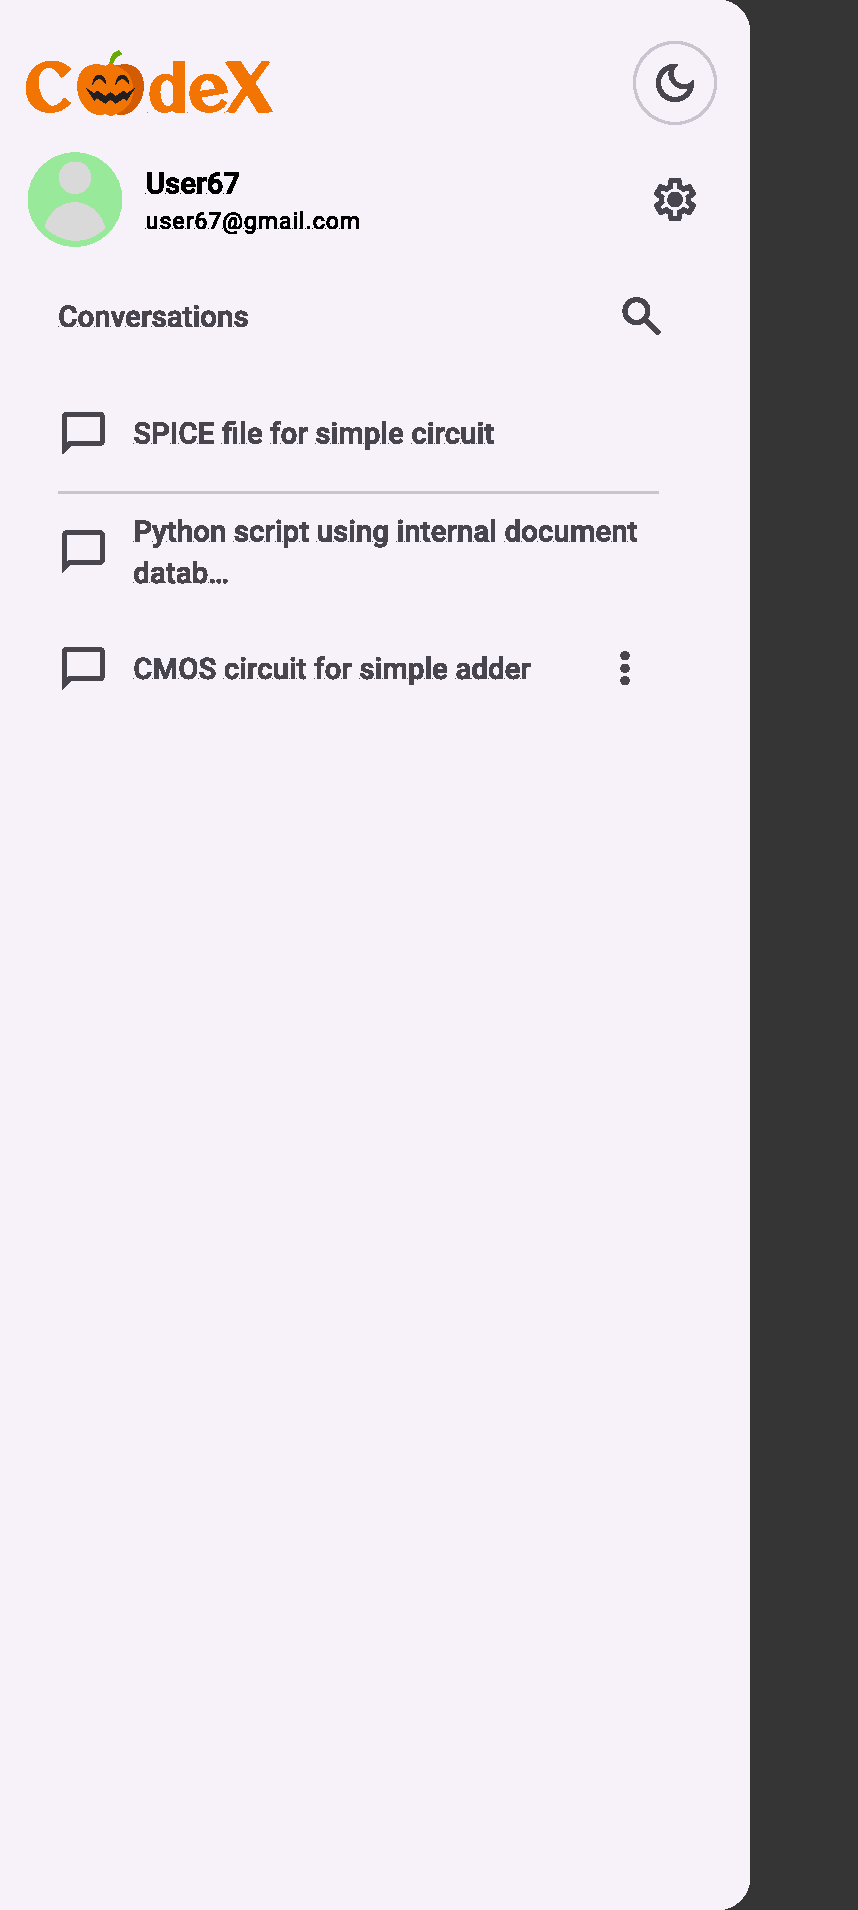
\includegraphics[width=6cm]{images/Navbar_Preview.pdf}
    \end{minipage}
\end{frame}


\begin{frame}[t]{User Interface}{Conversation Screen}
        \begin{itemize}
            \item<1-> Main screen of the app
            \item<2-> User can \textbf{enter the prompt}, \textbf{select language model} and \textbf{select the target language}
            \item<3-> After request is answered, generated code can be \textbf{viewed} or \textbf{visualized}.
        \end{itemize}
\end{frame}

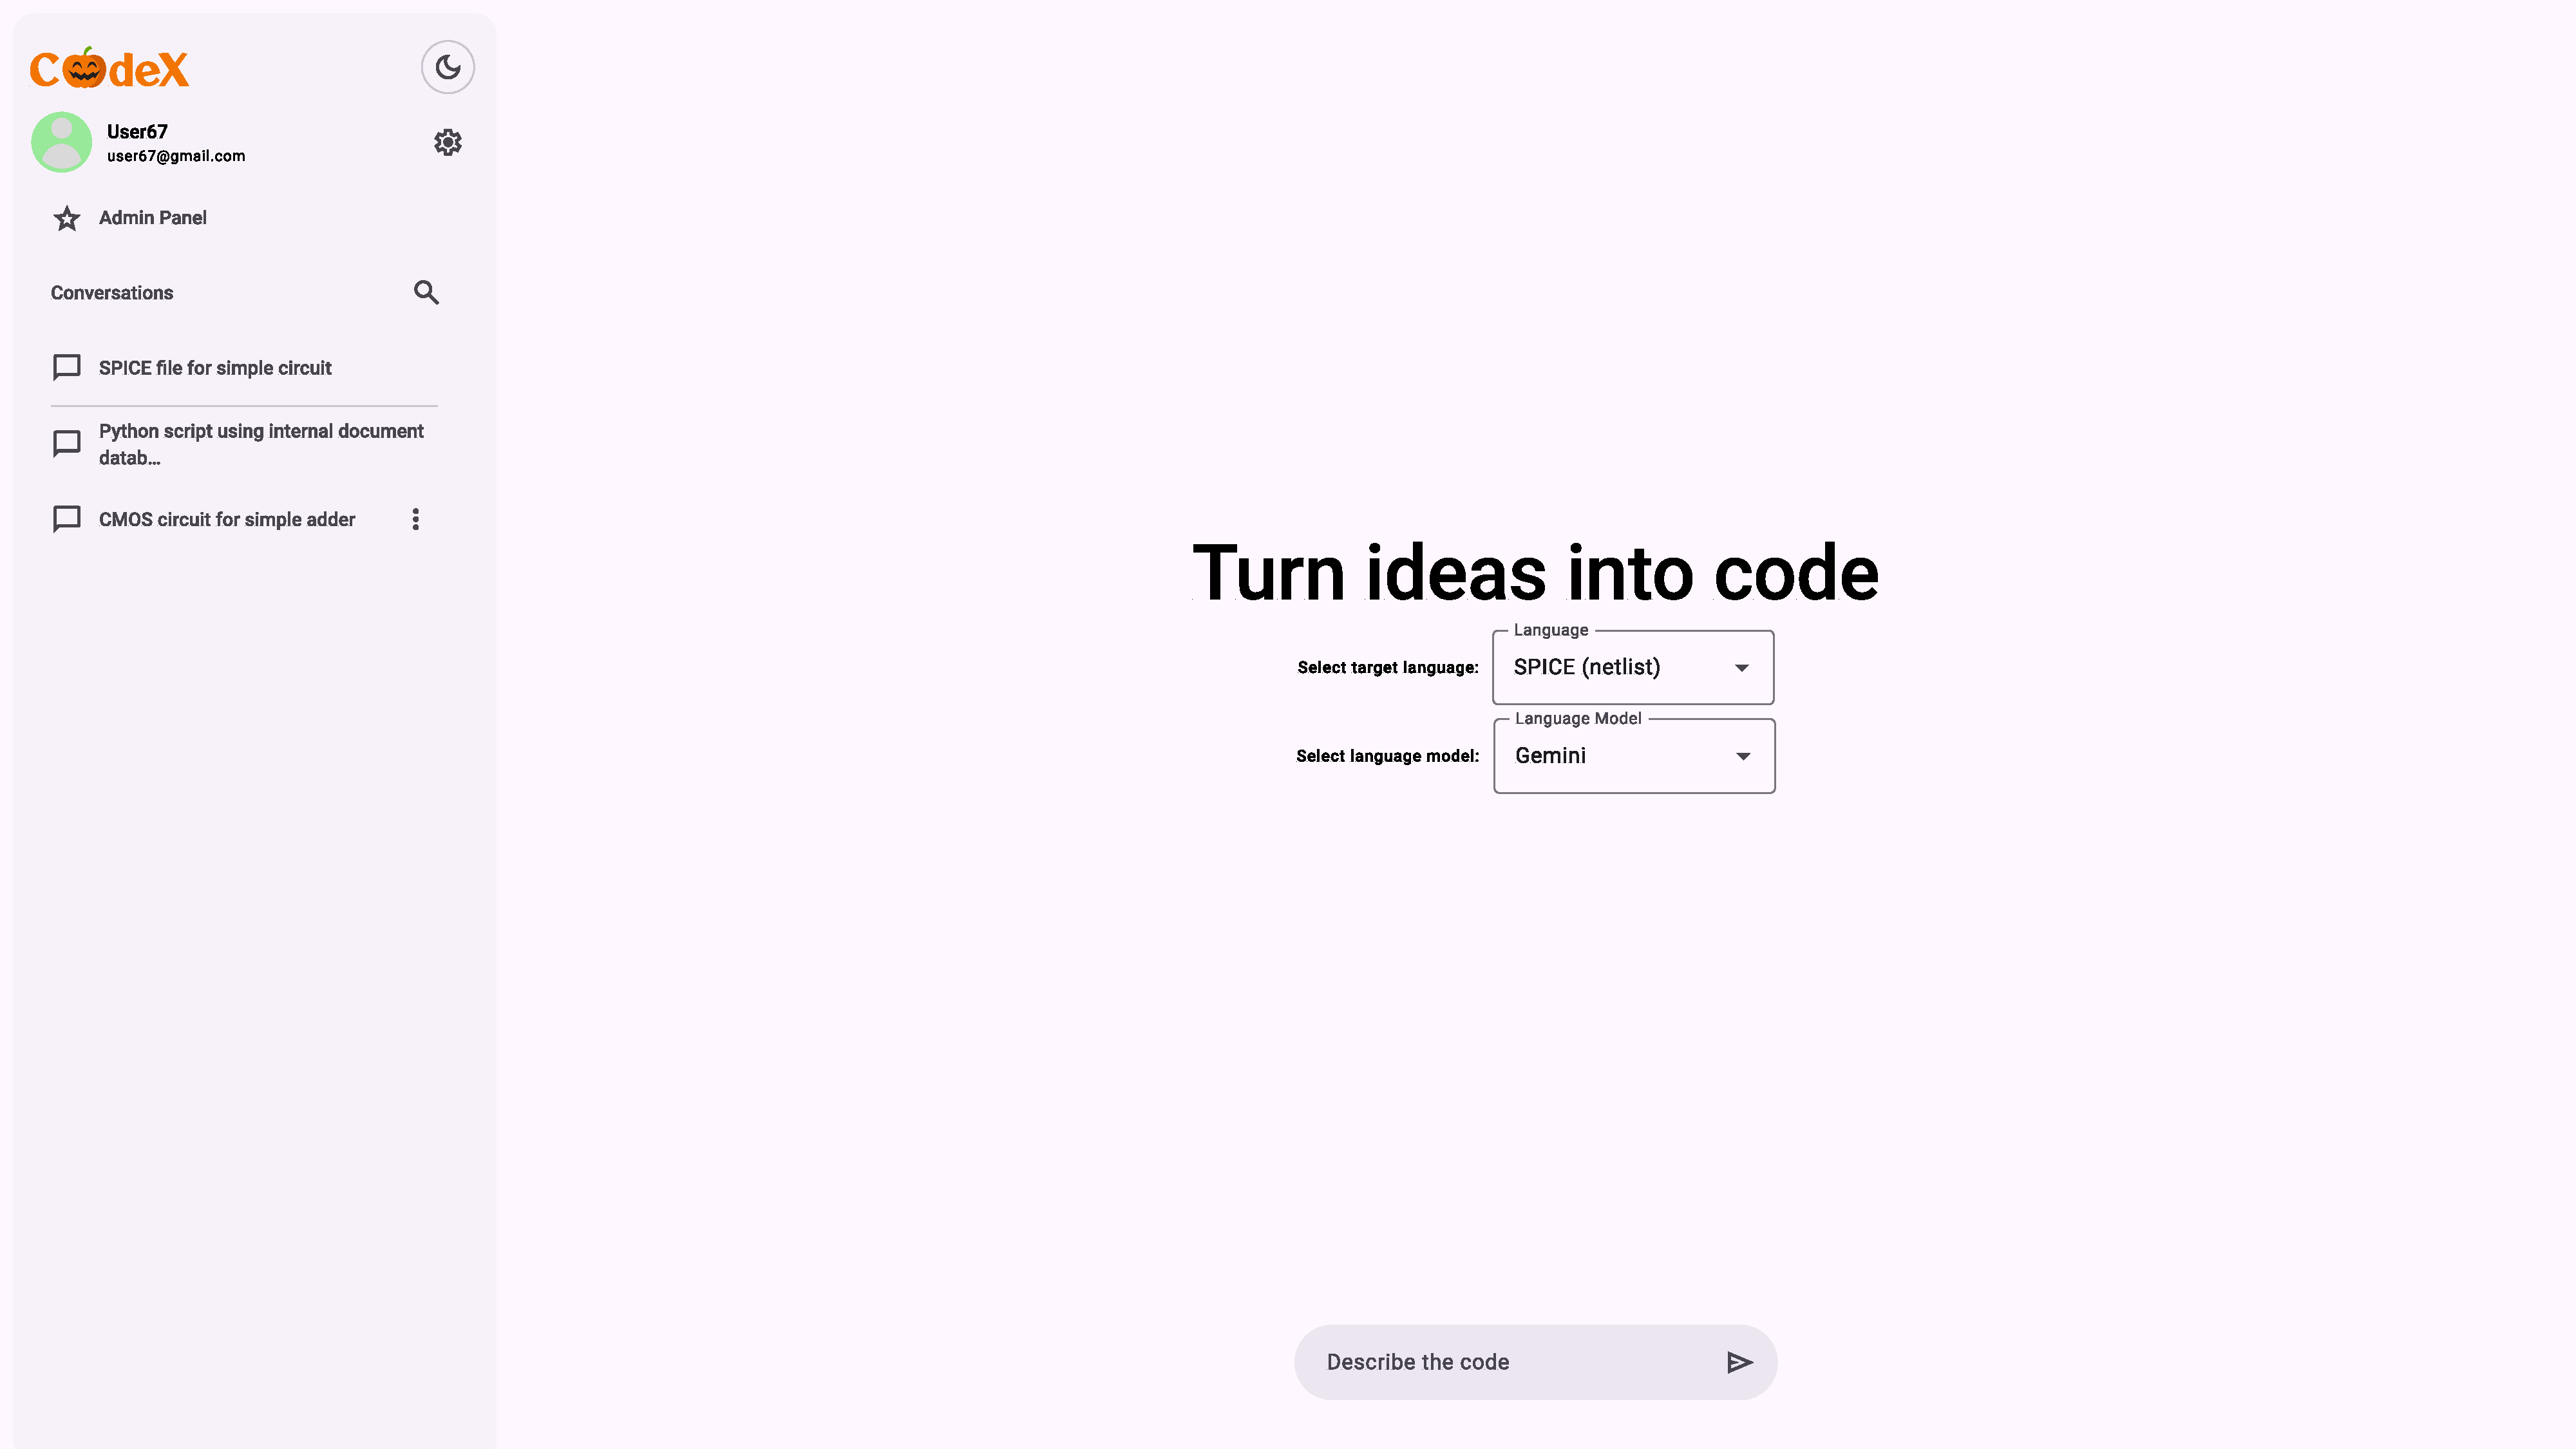
\includepdf{images/Conversation_Screen initial}
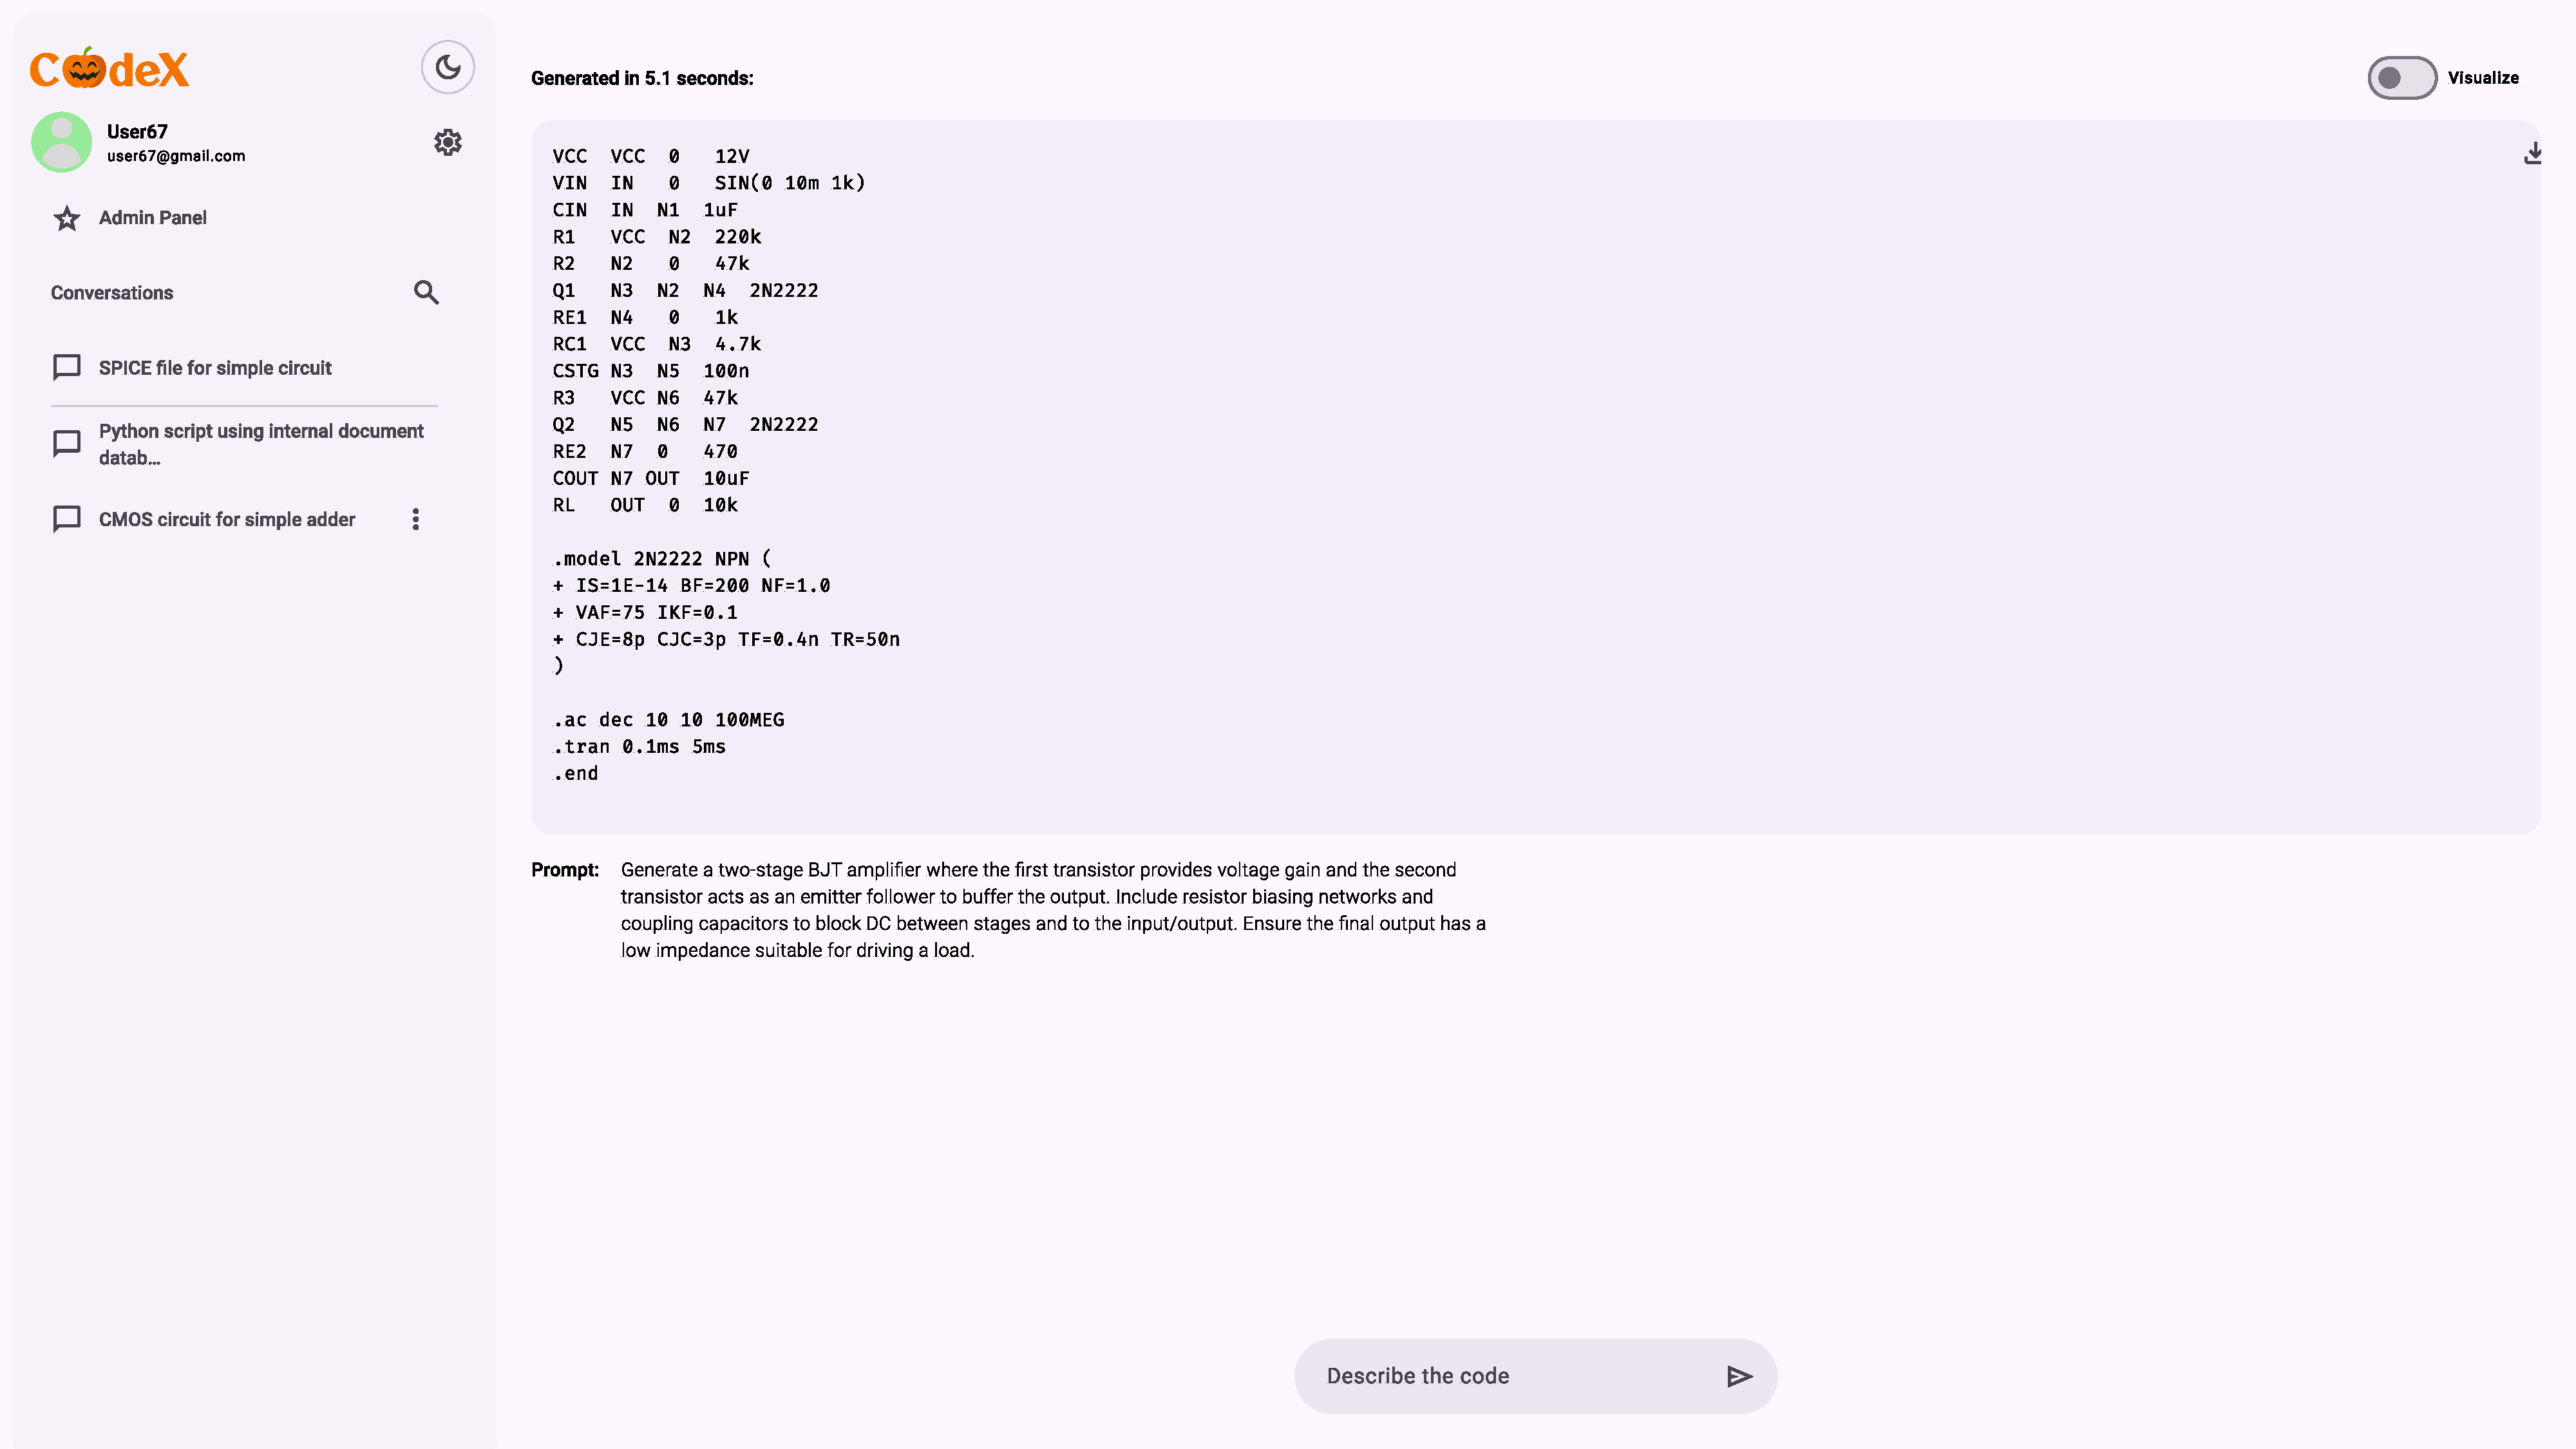
\includepdf{images/Conversation_Screen not-visualized}
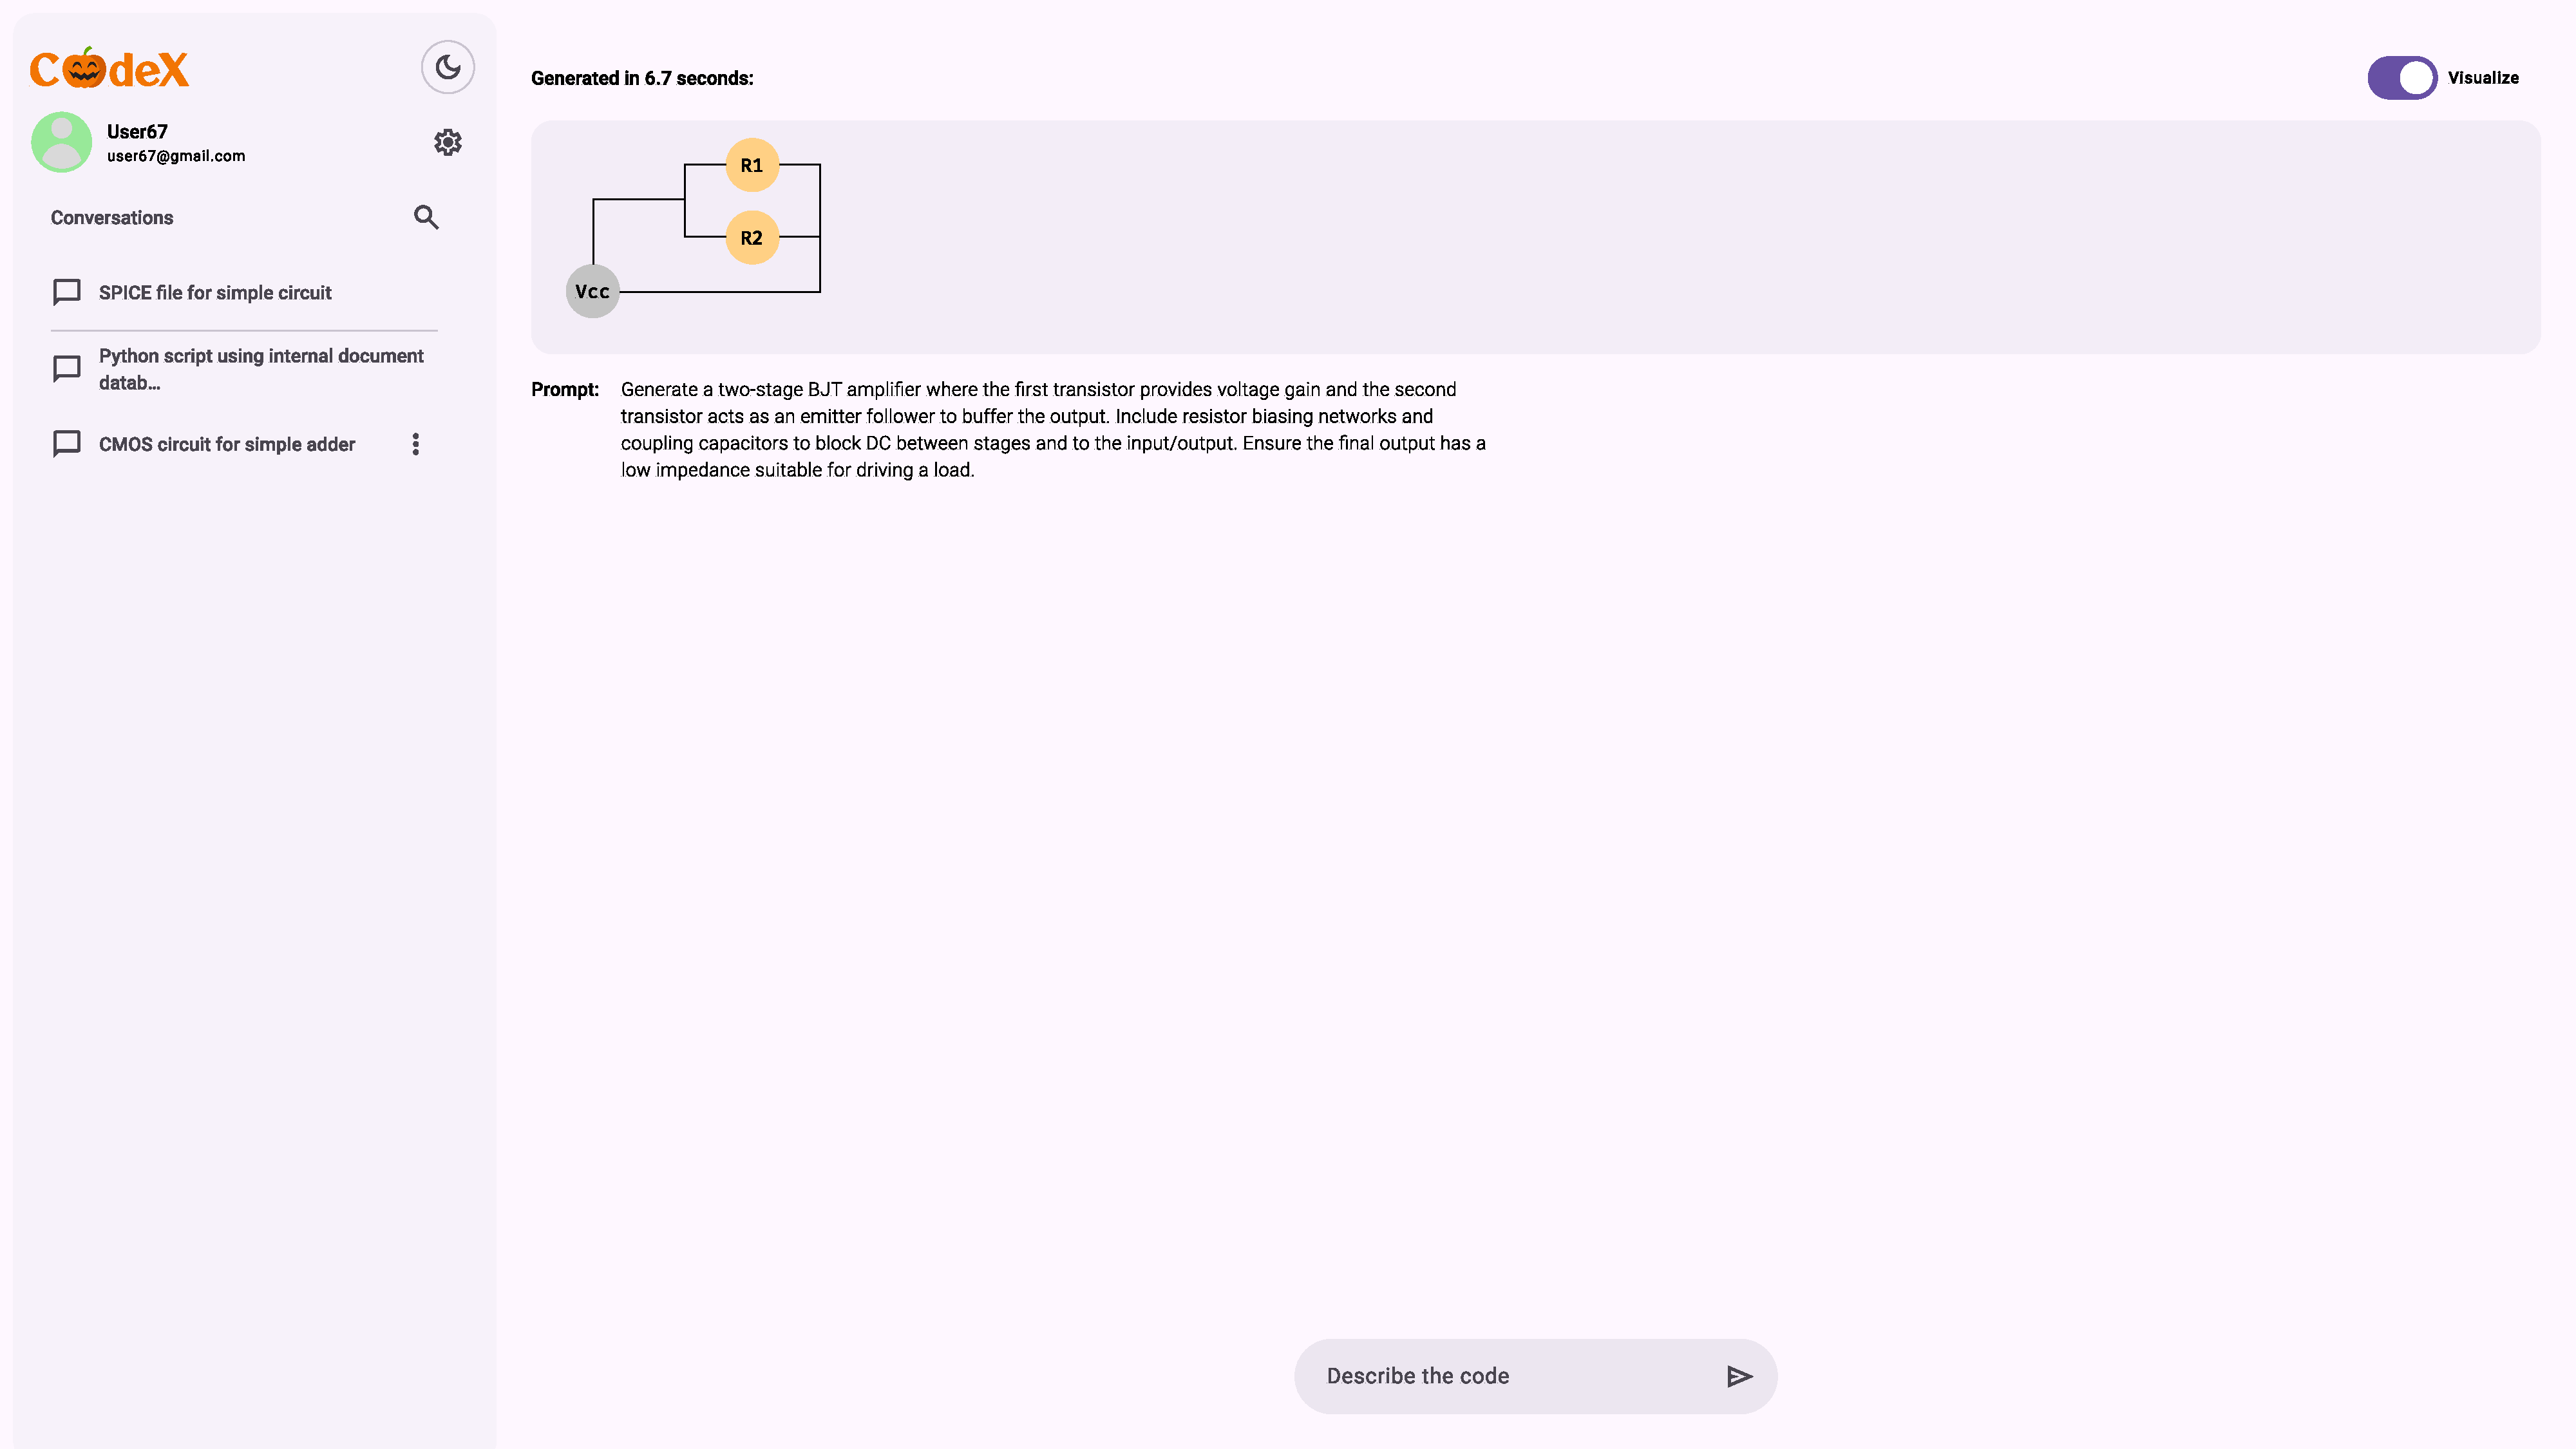
\includepdf{images/Conversation_Screen visualized}


\begin{frame}[t]{User Interface}{Authentication Screens }
        \begin{itemize}
            \item<1-> Authenticate via credentials by \textbf{logging in} or \textbf{signing up}
            \item<2-> Can navigate back-and-forth between both screens
            \item<3-> Optionally authenticate with an \textbf{OAuth provider} like google.
        \end{itemize}
\end{frame}

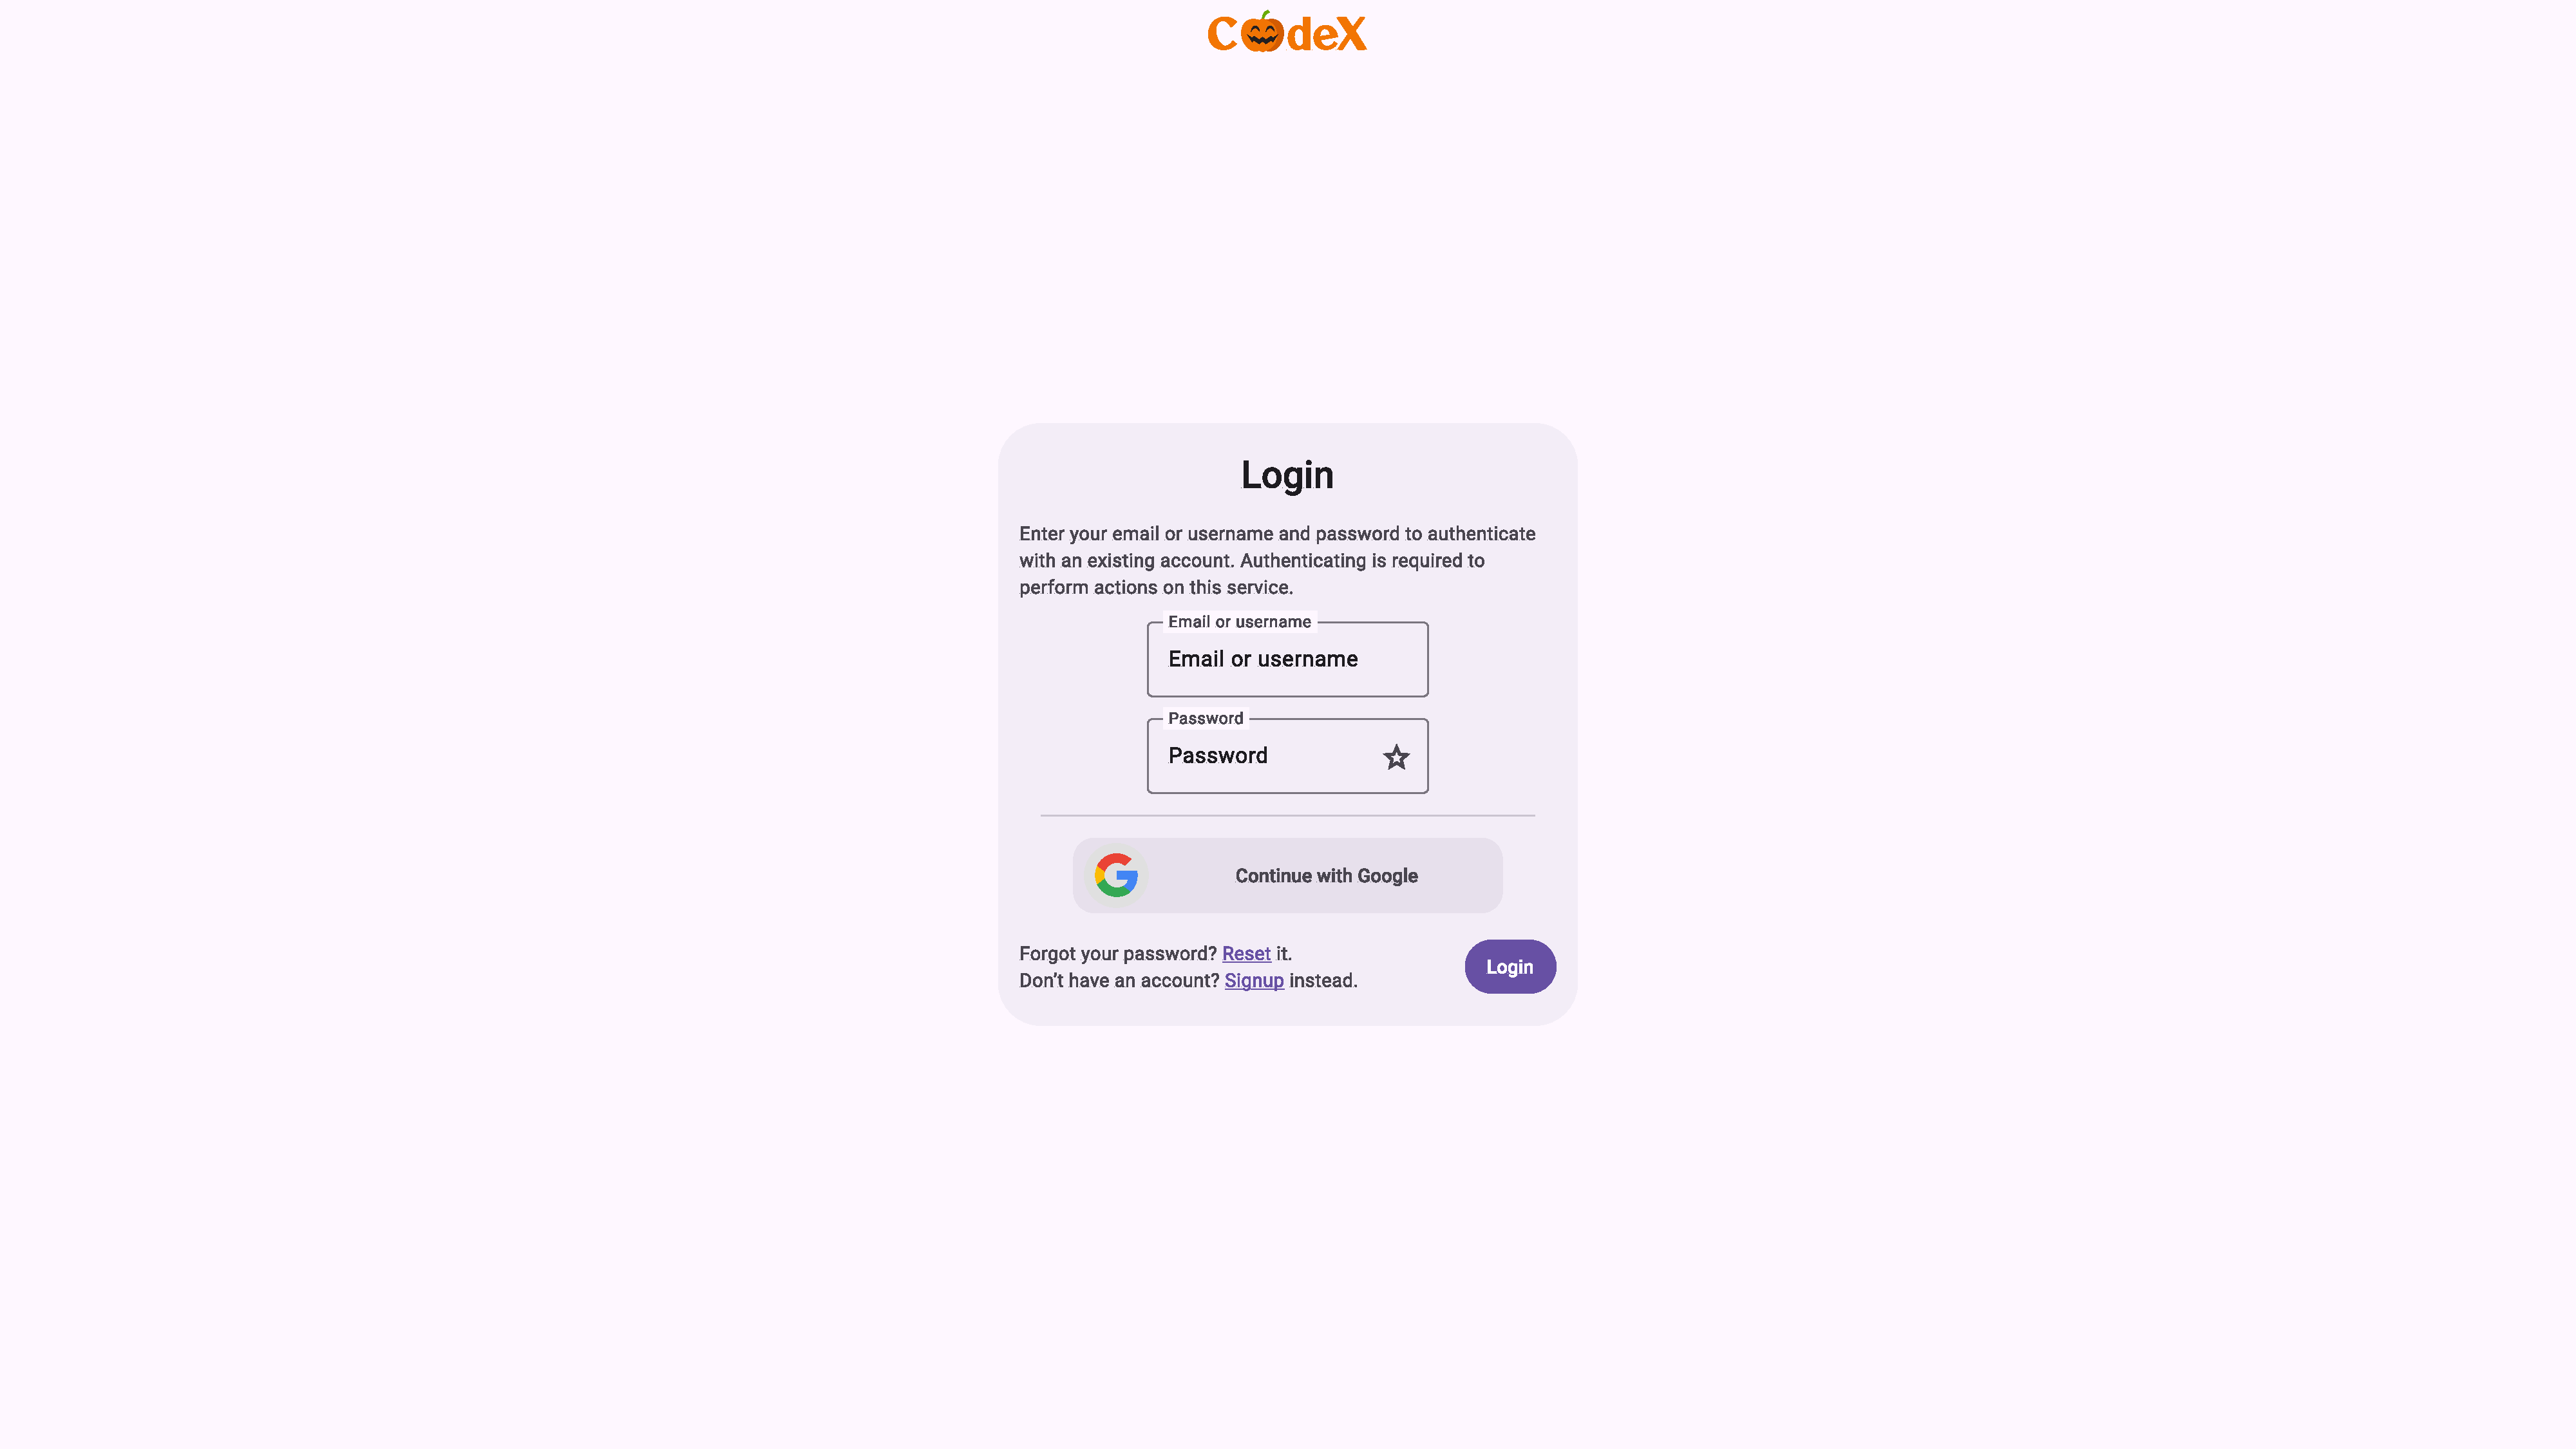
\includepdf{images/Login_Screen}
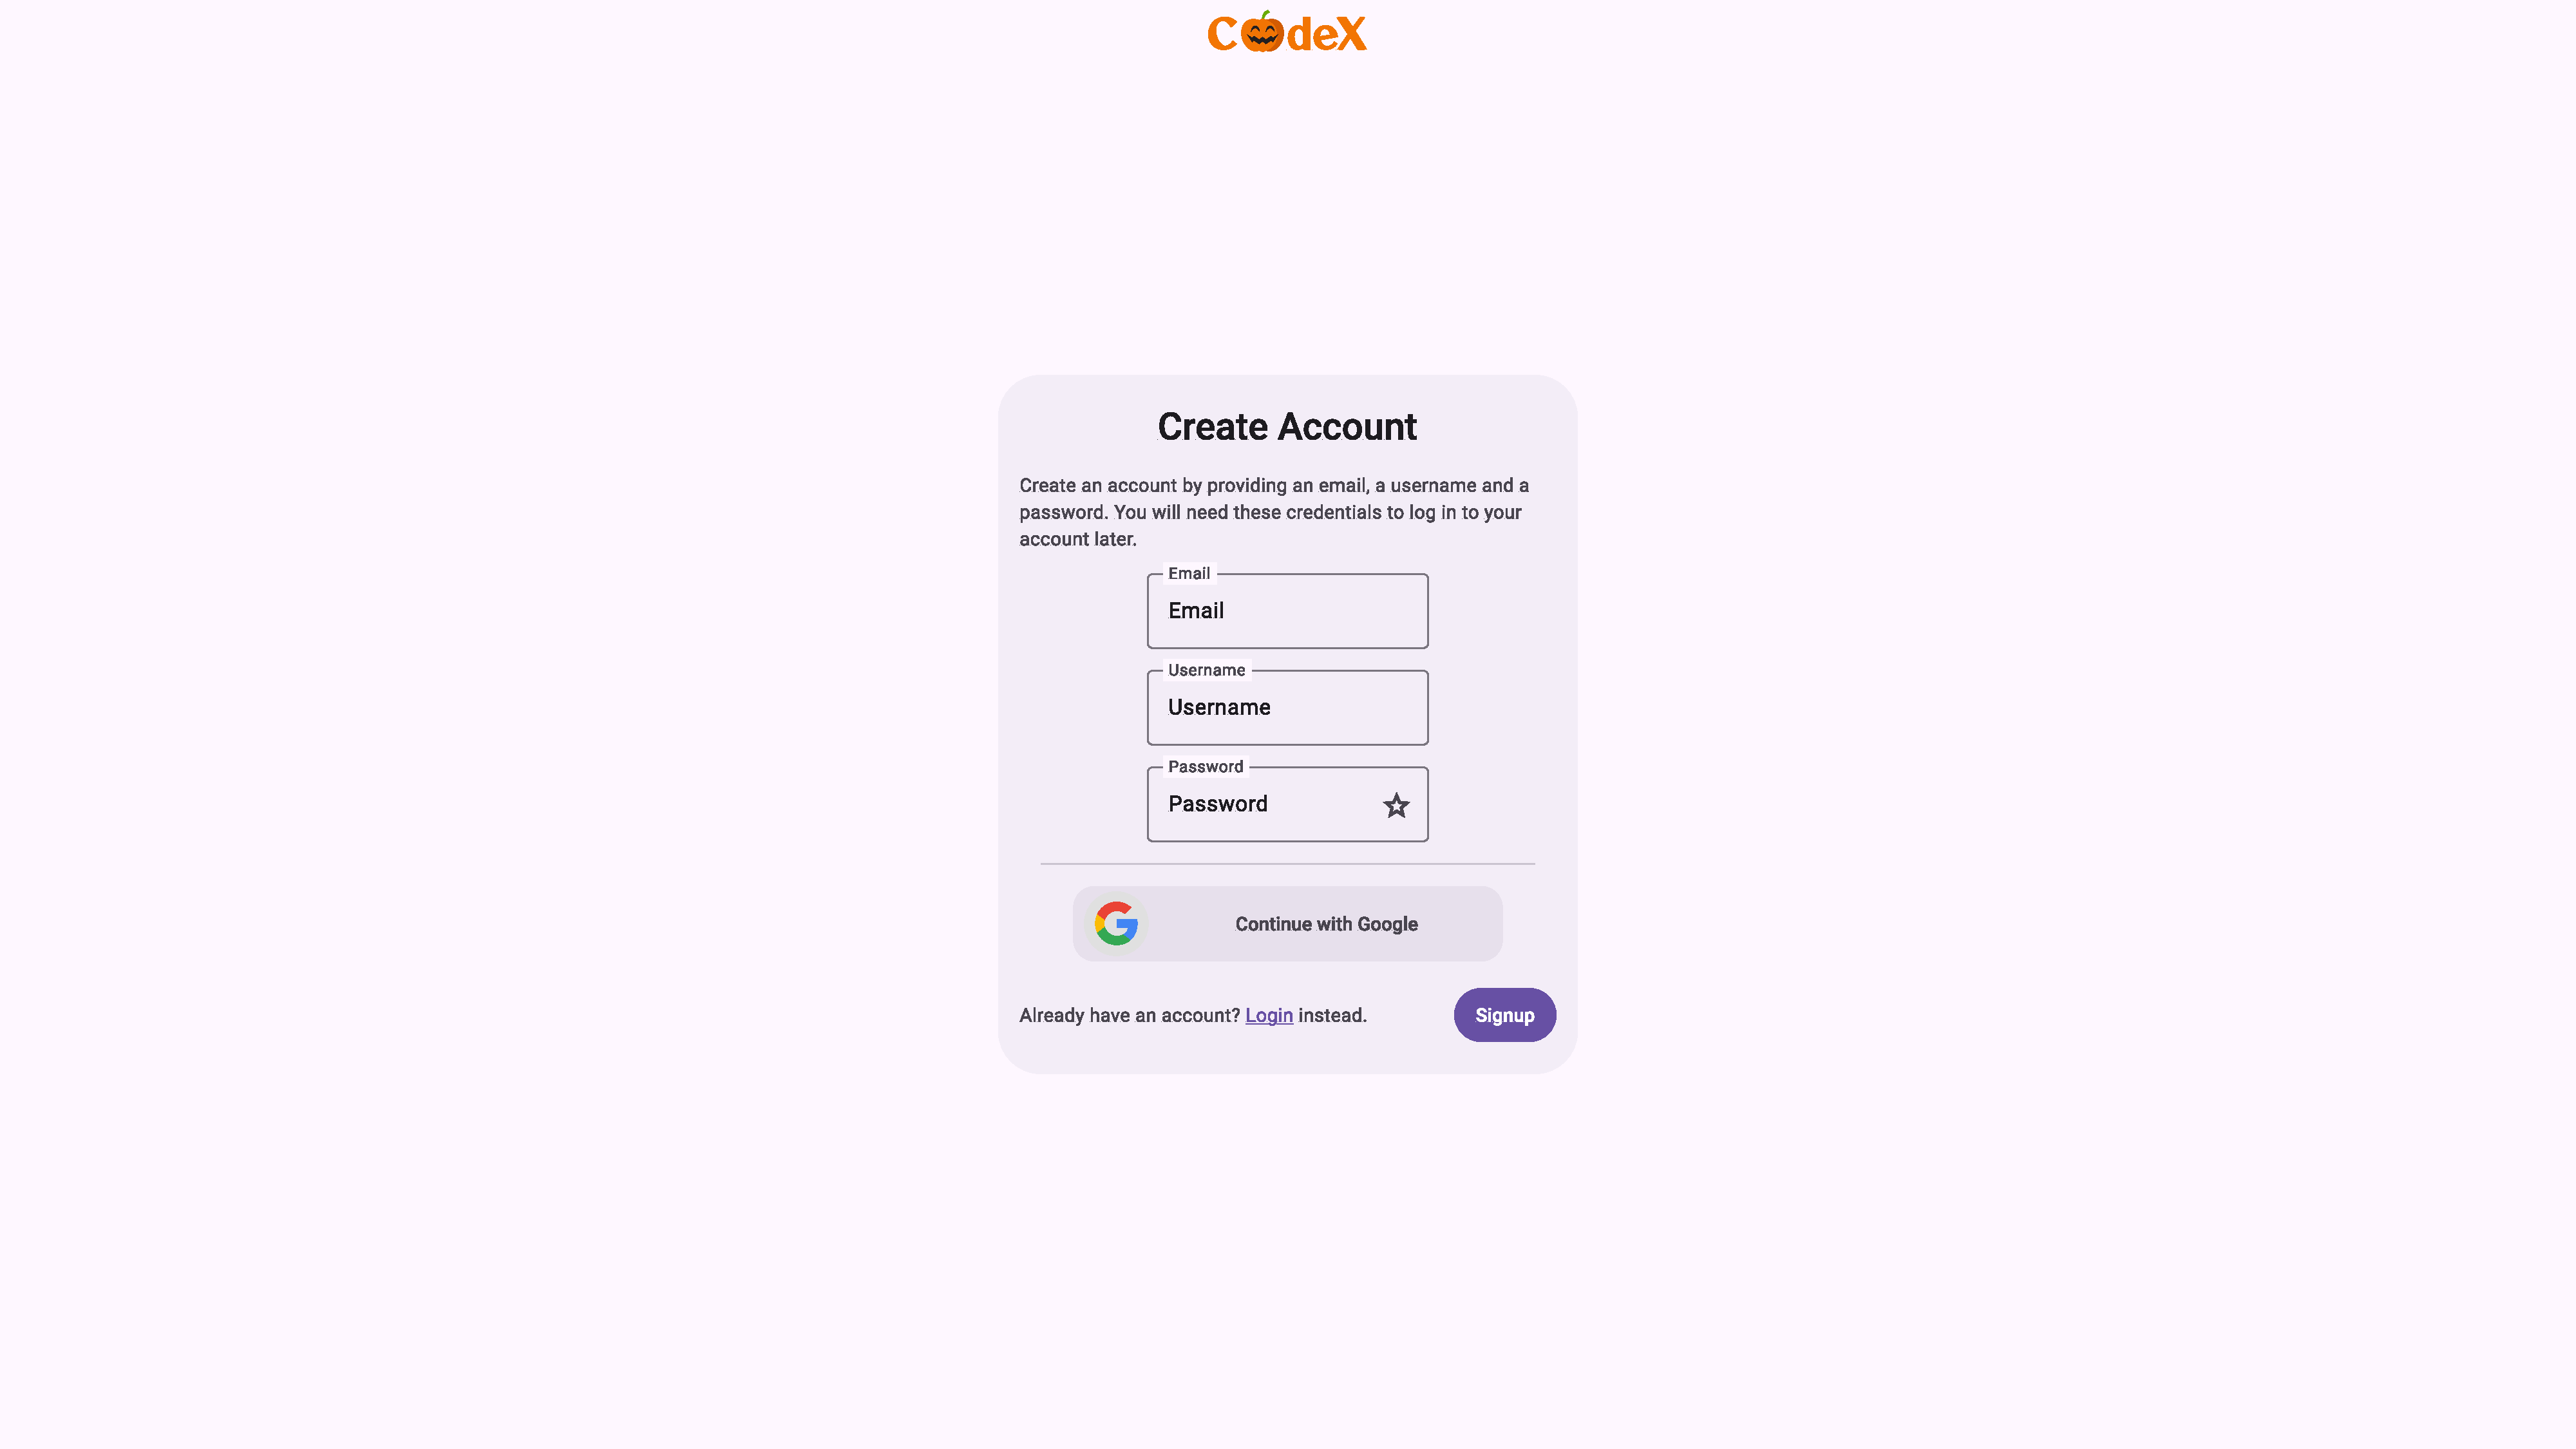
\includepdf{images/Signup_Screen}


\begin{frame}[t]{User Interface}{Admin Panel}
        \begin{itemize}
            \item<1-> Only accesisble to admins
            \item<2-> Main action: Set upper bounds for requests on a role-basis
            \item<3-> View basic analytics
        \end{itemize}
\end{frame}

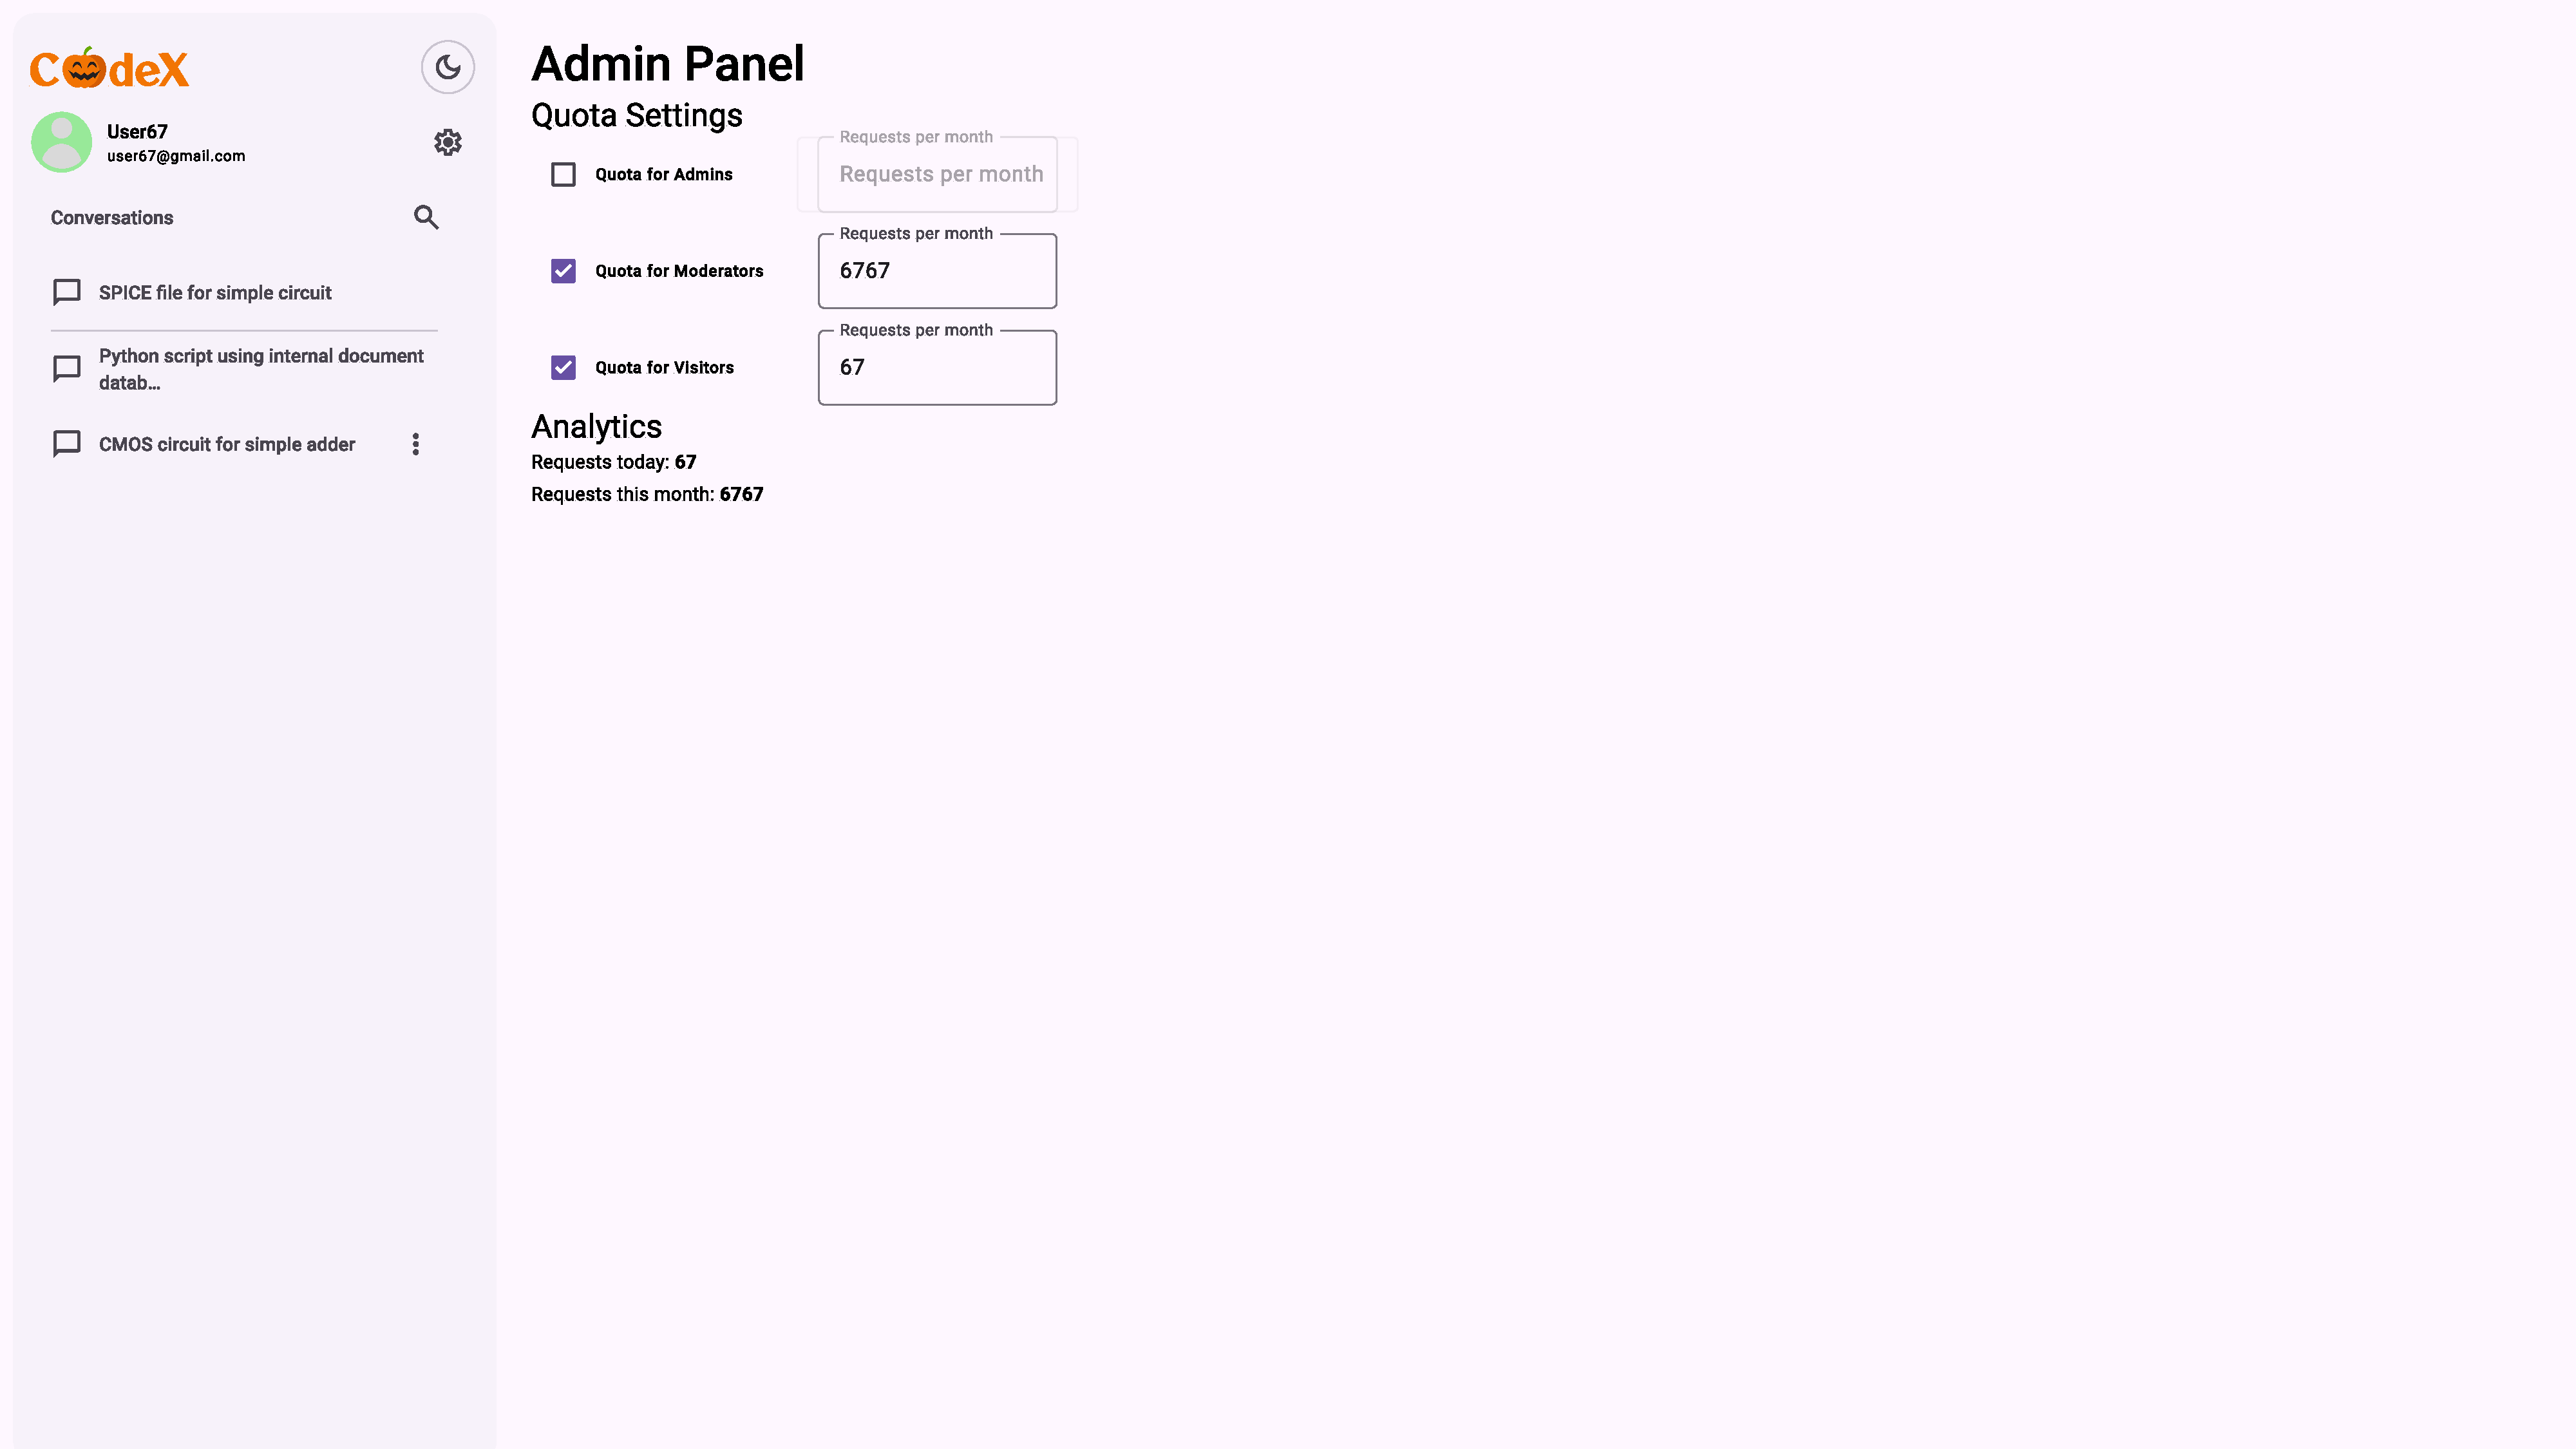
\includepdf{images/Admin_Panel_Screen}


\begin{frame}[t]{User Interface}{Settings Screen}
        \begin{itemize}
            \item<1-> Add, update or delete \textbf{LLM configurations}
            \item<2-> Stored on a user-basis, i.e. privately
        \end{itemize}
\end{frame}

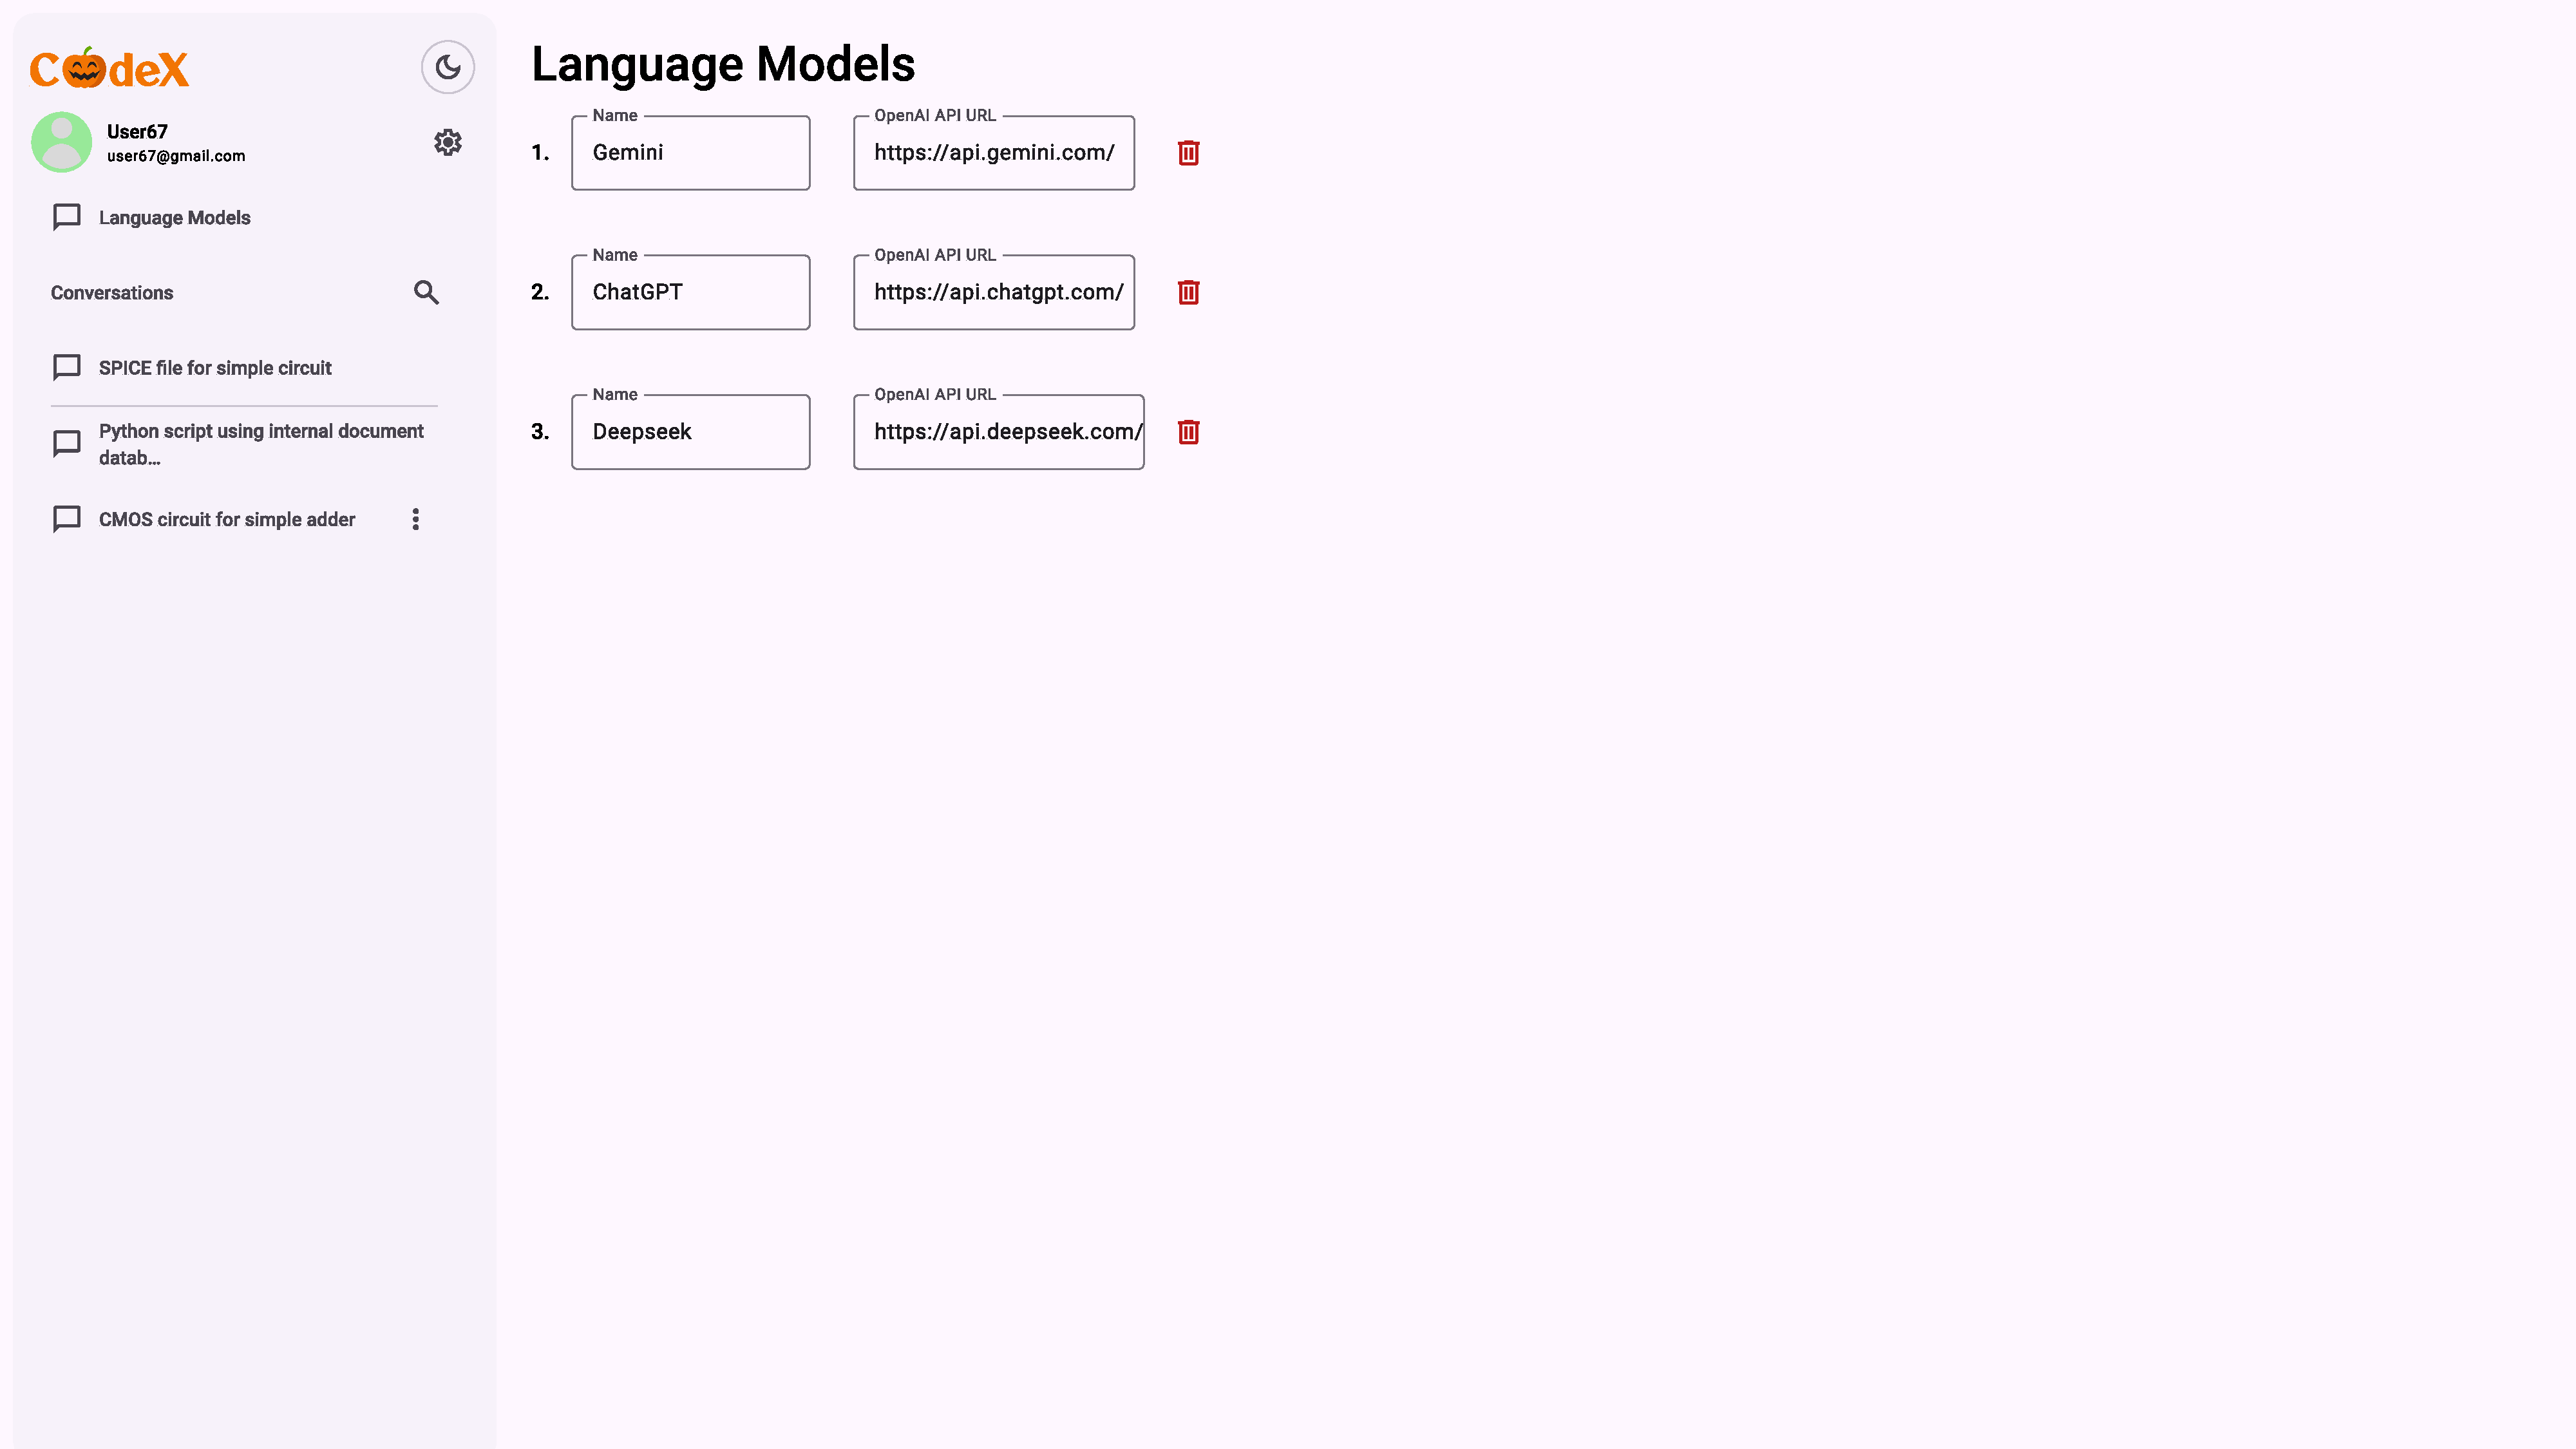
\includepdf{images/Settings_Screen}

\begin{frame}{}
    \textbf{Any further questions?}
\end{frame}

\end{document}
